\def\projectname{BrainBodyComputerInterface}
\def\documentname{SOFTWARE REQUIREMENTS\\ SPECIFICATION}

\def\authors{Maximilian Spahn}
\def\projectmembers{Ayberk Tuzcuoglu\\ Julian Emrich\\ Maximilian Spahn\\ Till Wolf}

\def\docversion{1.0 }
\def\docstatus{under construction} %(Status: = planned, under construction, presented, accepted)

\documentclass[a4paper]{scrreprt}

\usepackage{underscore}
\usepackage{hyperref}
\usepackage{lastpage}
\usepackage{float}
\usepackage{tikz}
\usepackage{tabularx}
\usepackage{longtable}
\usepackage[inkscapeformat=png]{svg}
\usepackage{scrlayer-scrpage}
\usepackage[utf8]{inputenc}
\usepackage[english]{babel}

\hypersetup{
    bookmarks=false,
    pdftitle={\projectname - \documentname},
    pdfauthor={\authors},
    colorlinks=true,
    linkcolor=blue,
    citecolor=black,
    filecolor=black,
    urlcolor=purple,
    linktoc=page
}

\rofoot*{}
\cofoot*{\thepage\ of {\hypersetup{linkcolor=black}\pageref{LastPage}}}
\pagestyle{scrheadings}

\begin{document}
\sffamily

\begin{titlepage}
	\begin{flushleft}
		\begin{LARGE}
			UNIVERSITY OF APPLIED SCIENCES \\ ASCHAFFENBURG
		\end{LARGE}
	\end{flushleft}

	\rule{15cm}{5pt}\vskip1cm

	\begin{flushright}
		\begin{bfseries}
			\begin{Huge}
				\documentname\\
				\vspace{1cm}
				for\\
				\vspace{1cm}
				\projectname\\
			\end{Huge}

			\vspace{1.2cm}

			\begin{Large}
				Version \docversion \docstatus\\
			\end{Large}
		\end{bfseries}

		\vspace{1.5cm}

		\begin{Large}
			\begin{bfseries}
				Author: \\
			\end{bfseries}
			\authors\\

			\vspace{1cm}

			\begin{bfseries}
				Project members: \\
			\end{bfseries}
			\projectmembers\\
		\end{Large}
		
		\vspace{1.5cm}

		\begin{bfseries} 
			\today\\ 
		\end{bfseries}

		\vspace{0.5cm}

		\small \bfseries{Documentname:}\\ \mdseries \textit{\jobname .tex}
	\end{flushright}
\end{titlepage}

\tableofcontents

\listoffigures

\chapter*{Revision History}

\begin{center}
    \begin{tabular}{|l|l|l|l|l|}
        \hline
		\bfseries{Version} & \bfseries{Status} & \bfseries{Creation Date} & \bfseries{Editor} & \bfseries{Modifications}\\
		\hline
		1.0 & under construction & 21.04.2023 & Maximilian Spahn & Initial version\\
        \hline
    \end{tabular}
\end{center}

\chapter{Introduction}

\section{Purpose}
This document describes the requirements and specifications for a game designed 
to showcase different bio-sensors. 
This document provides a detailed description of how the hardware 
should be used and what the game should do. 
While some specifications may be subject to change in later revisions, 
this document outlines the most important constraints.

\section{Scope}
Demonstrating the capabilities of technologies such as bio-sensors in a fun way is crucial 
to spark interest and development in this field. The game described in this document is 
intended to do exactly that. The goal of this project is to create a game that uses 
bio-sensors to control the game.\\

The game operates by selecting a random person from the audience, 
and the player must control a Moving Head to aim at the chosen person. 
The game then evaluates how well the player aimed at the target.

\section{Definition, Acronyms and Abbreviations}
\begin{longtable}{l l}
	API & Application Programming Interface\\
	fps & frames per second\\
	USB & Universal Serial Bus\\
	DMX & (Digital Multiplex) A protocol for controlling stage lighting\\
\end{longtable}

\section{References}
\begin{longtable}{l l}
	[AB-INF-PRC-1] & Programming guideline:\\
				   & Programmierrichtlinien für C/C++, Prof. Dr.-Ing. Konrad Doll, V 1.1\\
\end{longtable}

\section{Overview}
The SRS will specify in detail the software requirements for the "BrainBodyComputerInterface" product. 
Section 2 presents a general description of the product and it’s relationship within the operating environment (computer, external peripherals and sensors).
A complete list and description of the product functions and features will be provided. 
The type of user and user characteristics will be discussed. 
This Section also provides a discussion of any general constraints imposed on the product 
and any assumptions that are made regarding the operating environment of the product. \\

Section 3 will detail the software requirements of the "BrainBodyComputerInterface" product. 
The behavioral requirements of the software and operating environment will be discussed.
The external interface, the hardware interfaces, the software interfaces, and the
communication interfaces of the product will be outlined. 
Performance requirements will be discussed in section 3. 
Included in this discussion are operational requirements, exception handling, and testing requirements. 
Design constraints concern for the design phase of the product development will be addressed. 
Section 3 also describes the following product attributes: availability, security, maintainability, transferability and portability.

\chapter{General Description}
This chapter describes the general description of the product.

\section{Product Perspective}
The main part of the product is a game that uses bio-sensors to control the game.
Therefore the software will have to communicate with the different sensors and their corresponding 
APIs or any other software that is needed to use the sensors.
Also the software will have to communicate with a webcam to get view of the audience and a Moving Head to aim at the target.
Aside from the sensors and the webcam, there game will only require a mouse and a keyboard to be played.
Any other input devices like gamepads or a joysticks are not intended to be used.

\begin{figure}[H]
	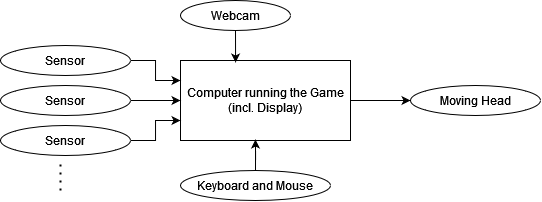
\includegraphics[width=10cm]{hardware_and_peripherals}
	\centering
	\caption{Hardware and Peripherals Overview}
	\centering
	\label{fig:brainbodycomputerinterface}
\end{figure}

\section{Product Functions}
The game will have to fulfill the following functions:
\begin{itemize}
	\item communicate with the different sensors
	\item interpret the data from the sensors and use it to control the Moving Head
	\item communicate with the webcam and select a random person from the audience
	\item display the camera view on the screen
	\item overlay a simple user interface on the camera view
	\item the user interface will display the current score and the current target and other information
\end{itemize}

\section{User Characteristics}
The software is intended to be mostly used as demonstration software for the bio-sensors.
Therefore the software will mostly used by the person who is demonstrating it.
It can be assumed that only the person demonstrating the software, in this case the lecturer, 
must be familiar with it and be able to fully understand its settings and functions.
Nevertheless, the user interface while playing, should also be simple and easy to understand for the person trying out the game.

\section{General Constraints}
The language of all documents, the code and the GUI is english. A usage of Open Source
packages is possible.

\section{Assumptions and Dependencies}
The software will be developed for Windows 10 and 11. 
Keeping compatibility with other operating systems is not a priority but it is not excluded either. (Support for Linux is planned but has no priority. Support for MacOS is not planned and mostly not possible.) \\
The software will use Vulkan and SDL and therefore will require a graphics card that supports Vulkan, which is the case for most modern graphics cards.

\chapter{Specific Requirements}

\section{Gameplay}

\begin{itemize}
	\item When the game starts the player will be presented with a camera view of the audience. \\
	\item The game will then select a random person from the audience as a target and mark the person on the webcam feed. \\
	\item The player will then have to aim the Moving Head at the target. \\
	\item The player will be able to move the Moving Head around by using various bio-sensors. \\
	\item The game will then evaluate how well the player aimed at the target and give the player a score. \\
\end{itemize}

\subsection{winning condition}
The game will end when the player manages to aim the Moving Head at the target.
\subsection{losing condition}
The game will end when the player fails to aim the Moving Heads beam at the target in a certain amount of time.
\subsection{difficulty}
The difficulty of the game will be determined by the amount of time the player has to aim the Moving Head at the target.
\subsection{highscore}
The game will keep track of the highscore and display it on the screen.

\section{Functional Requirements}
The to run the above described gameplay the software will have to fulfill the following functional requirements:

\subsection{Selecting the difficulty}
\begin{longtable}{ l p{12cm}}
	Input: & The game reads the user input from the keyboard and mouse.\\
	Description: & Before starting the game the player will be able to select the difficulty of the game.\\
\end{longtable}

\subsection{Starting the game}
\begin{longtable}{ l p{12cm}}
	Input: & The game reads the user input from the keyboard and mouse.\\
	Description: & When the player starts the game, the above described gameplay will be started.\\
\end{longtable}

\subsection{Displaying the camera view}
\begin{longtable}{ l p{12cm}}
	Input: & The game reads the video stream from the webcam.\\
	Output: & The game displays the camera view on the screen.\\
	Description: & The game will display the camera view on the screen.\\
\end{longtable}

\subsection{Selecting a random person from the audience}
\begin{longtable}{ l p{12cm}}
	Input: & The game reads the video stream from the webcam.\\
	Output: & The game selects a random person from the audience as a target and mark the person on the webcam feed.\\
	Description: & When starting the game the game will select a random person from the audience as a target.\\
\end{longtable}

\subsection{Control of the Moving Head}
\begin{longtable}{ l p{12cm}}
	Input: & The game reads the data from the Sensors and interprets it.\\
	Output: & The game controls the Moving Head. The game will have to control the panning, tilting, size, gobo and shutter of the Moving Head.\\
	Description: & To enable the user, aiming the beam at the target, the game will read the data from the sensors and use it to control the Moving Head. How the data from the sensors is used to control the Moving Head is not specified and depends on the sensors.\\
\end{longtable}

\subsection{Evaluating the aiming}
\begin{longtable}{ l p{12cm}}
	Input: & The game detects the position of the target and the position of the Moving Head.\\
	Output: & The game displays the current score on the screen.\\
	Description: & The game will evaluate how well the player aimed at the target and give the player a score.\\
\end{longtable}

\subsection{Pausing and resuming the game}
\begin{longtable}{ l p{12cm}}
	Input: & The game reads the input from the keyboard and mouse.\\
	Description: & The game will pause or resume the game when the user presses the space bar or presses the pause button on the user interface.\\
\end{longtable}

\section{External Interface Requirements}
\subsection{User Interface Requirements}
After starting the game the user interface will be a simple menu.
The menu will have a button to start the game, a button to quit the game and a button to change the difficulty.
While playing the game the user interface will be a simple overlay on the camera view.
The user interface will display the current target and the current score.
Also the user interface will display a button to pause the game.
From the pause menu the user will be able to resume the game or quit the game.
Other than this there are no specific requirements or constraints for the user interface.

\subsection{Hardware Interface Requirements}
\subsubsection{Sensors}
How the sensors are connected to the computer will be determined by the sensors.
For now its not determined what sensors will be used, and therefore no specific requirements or constraints for the sensors are specified yet.

\subsubsection{Webcam}
The webcam will be a standard webcam, which will interface with the computer via USB.

\subsubsection{Moving Head}
The Moving Head will be controlled via the DMX protocol.
The DMX protocol is a serial protocol that writes data to different channels.
The used channels will be determined by functionality of the Moving Head.
The Moving Head will have to be connected to a DMX controller, which will be connected to the computer via USB.

\subsection{Software Interface Requirements}
The software will use the Vulkan graphics API to render the camera view and the user interface.
Other than this are no specific requirements or constraints for the software interface.

\subsection{Communications Interface Requirements}
Unless the hardware somehow requires it, the software will not communicate with any other software or hardware.

\section{Performance Requirements}
The software will have to provide a fluid and responsive experience.
Therefore the software will have to be able to run at a minimum of 30 frames per second and 60fps on average on a modern (normal spec) computer.
Also the update rate for the sensors should be at least 30 Hz. (if the sensor supports it, otherwise the maximum supported update rate)

\section{Design Constraints}
\subsection{Standards Compliance}
The code follows the programming guidelines described in [AB-INF-PRC-1].

\subsection{Hardware Limitations}
The software is designed to run on x86-64 architecture computers. Either a integrated or a dedicated graphics card is supported as long as it supports Vulkan 1.2.

\section{Software System Attributes}
\subsection{Distribution}
While here are no specific requirements for the distribution 
of the software, its aimed to be distributed as a folder containing 
all the necessary files and executables to run the software 
on a Windows 10 or 11 computer.

\subsection{Deployment}
The software is only planned to be used on a single computer, 
which is used to demonstrate software projects like this one.
But it should still be easy to deploy the software on other computers.

\subsection{Adding Sensors}
While its not required to later add more sensors after the project 
is completed and handed over, it should be possible to do so.
Therefor the code handling the sensors should be written in a way 
that makes it easy to add more sensors. 
(This will also make it easier to react to any changes in the software requirements.)

\section{Other Requirements}
Other requirements do not apply to this project.

\end{document}
